\documentclass[border=10pt]{standalone}
\usepackage{tikz}\usepackage{amsmath}\usetikzlibrary{arrows.meta}
\begin{document}
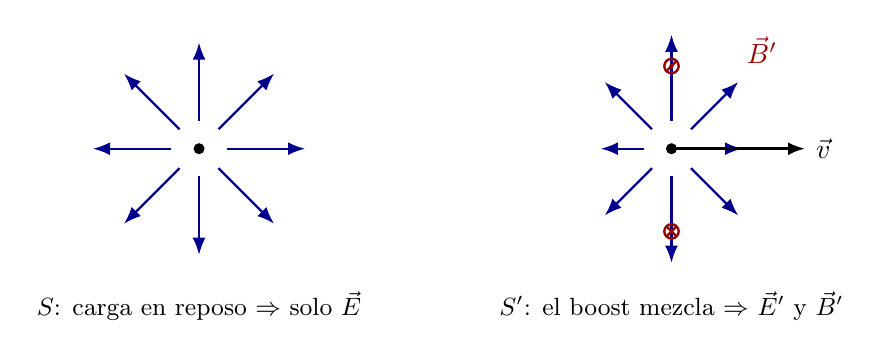
\begin{tikzpicture}[line width=0.85pt,>={Latex[length=2.2mm]}]
  % S: carga en reposo, solo E
  \fill (0,0) circle(2pt);
  \foreach \a in {0,45,...,315} \draw[->,blue!55!black] (\a:0.35)--(\a:1.35);
  \node at (0,-2.0){\small $S$: carga en reposo $\Rightarrow$ solo $\vec E$};
  % S': carga en movimiento, E' y B'
  \begin{scope}[xshift=6cm]
    \fill (0,0) circle(2pt);
    % E' comprimido (mas fuerte perpendicular)
    \foreach \a/\l in {0/0.9,45/1.2,90/1.45,135/1.2,180/0.9,225/1.2,270/1.45,315/1.2}
       \draw[->,blue!55!black] (\a:0.35)--(\a:\l);
    \draw[->,line width=1.1pt] (0,0)--(1.7,0) node[right]{$\vec v$};
    % B' (saliente arriba, entrante abajo)
    \draw[red!60!black] (0,1.05) circle(2.6pt); \fill[red!60!black] (0,1.05) circle(0.8pt);
    \draw[red!60!black] (0,-1.05) circle(2.6pt); \draw[red!60!black] (-0.07,0.98)--(0.07,1.12);
    \draw[red!60!black] (-0.07,-1.12)--(0.07,-0.98)(-0.07,-0.98)--(0.07,-1.12);
    \node[red!60!black] at (1.15,1.25){$\vec B'$};
    \node at (0,-2.0){\small $S'$: el boost mezcla $\Rightarrow$ $\vec E'$ y $\vec B'$};
  \end{scope}
\end{tikzpicture}
\end{document}
